\documentclass[twoside,leqno, 11pt]{article}

\usepackage[svgnames, table]{xcolor}
\usepackage{cmap}
\usepackage{graphicx} 
\usepackage{wrapfig}
\usepackage{lastpage}
\usepackage{tikz}
\usepackage{multirow}
\usetikzlibrary{calc}
\usepackage{pgfplots}
\pgfplotsset{width=7cm,compat=1.8}
\usepackage{braket}
\usepackage{verbatim}
\usetikzlibrary{arrows}
\usetikzlibrary{calc,positioning,fit,backgrounds}
\usetikzlibrary{decorations.pathreplacing,calc}
\usepackage{amsmath} 
\allowdisplaybreaks
\usepackage[T2A]{fontenc}
\usepackage[utf8]{inputenc}	
%\usepackage[english,russian]{babel}
\usepackage{geometry}
\geometry{top=16mm}
\geometry{bottom=16mm}
\geometry{left=16mm}
\geometry{right=16mm}	
\usepackage{amssymb}
\usepackage{listings}
\lstset{language=R,
    basicstyle=\small\ttfamily,
    stringstyle=\color{DarkGreen},
    numberstyle=\tiny\color{DarkRed}, 
    rulecolor=\color{black},
    morekeywords={TRUE,FALSE},
    deletekeywords={data,frame,length,as,character},
    keywordstyle=\color{DarkBlue},
    commentstyle=\color{DarkGreen},
}       
\usepackage{icomma} 
\usepackage{mathtext} 
\usepackage{mathrsfs}
\usepackage{mathtools}
\usepackage{fancyhdr}
\pagestyle{fancy}
\fancyhf{}
\renewcommand{\headrulewidth}{0,04mm}
\usepackage{hyperref}
\usepackage{mathtext} 
\usepackage{multicol}
\chead{\scshape{Tutorial on Active Inference \\ Весна 2020}}
%\lhead{}
%\chead{\date{\today}} 
\cfoot{\thepage} 
%\hypersetup{
%  colorlinks=true
%   linkcolor=red,       
%        citecolor=black,   
%        filecolor=magenta, 
%        urlcolor=blue}
\makeatletter % сделать "@" "буквой", а не "спецсимволом" - можно использовать "служебные" команды, содержащие @ в названии
\renewcommand{\headrulewidth}{0,6mm} 

\renewcommand{\maketitle}{\begin{center}
	\noindent{\bfseries\scshape\LARGE\@title}\par
\noindent {\large\scshape\bfseries\@subtitle}\par
\noindent {\large\slshape\mdseries\@author}
\vskip 2ex
\end{center}}

\DeclareMathOperator*{\plim}{plim}
\DeclareMathOperator{\var}{Var}
\newcommand{\lag}{\mathcal{L}}
\newcommand{\e}{\mathbb{E}}
\newcommand{\p}{\mathbb{P}}
\newcommand{\n}{\mathcal{N}}


\pgfmathdeclarefunction{gauss}{2}{%
        \pgfmathparse{1/(#2*sqrt(2*pi))*exp(-((x-#1)^2)/(2*#2^2))}%
    }

\renewcommand{\maketitle}{\noindent{\bfseries\scshape\LARGE\@title}\par
        
\noindent {\slshape\mdseries\@author}
\vskip 2ex}

\renewcommand\section{\@startsection{section}{1}{\z@}%
        {-3.5ex \@plus -1ex \@minus -.2ex}%
        {-1em}%
        {\normalfont\large\scshape\bfseries}}

%\renewcommand\subsection{\@startsection{subsection}{1}{\z@}%{-3.5ex \@plus -1ex \@minus -.2ex}%       {-1em}%{\normalfont\bfseries}}
\renewcommand*\env@matrix[1][*\c@MaxMatrixCols c]{%
  \hskip -\arraycolsep
  \let\@ifnextchar\new@ifnextchar
  \array{#1}}
  \newenvironment{sqcases}{%
  \matrix@check\sqcases\env@sqcases
}{%
  \endarray\right.%
}
\def\env@sqcases{%
  \let\@ifnextchar\new@ifnextchar
  \left\lbrack
  \def\arraystretch{1.2}%
  \array{@{}l@{\quad}l@{}}%
}
\makeatother

%\title{Problem Set 2}
\author{Махнева Елизавета, Брсикян Бабкен \\ БЭК171}

\begin{document}
\maketitle
	
\section*{Предисловие от авторов}~\

	Данная статья является переводом \href{https://medium.com/@solopchuk/tutorial-on-active-inference-30edcf50f5dc}{Tutorial on Active Inference} Олега Солопчука. Так как тема Свободной Энергии является достаточно новой в научной среде, в этой статье присутствует много терминов, которые не очень популярны, с которыми русский читатель встречается впервые. В связи с чем очень тяжело перевести их на русский язык точно, потому что в русском языке такие словосочетания и слова не имеют определенного смысла. Но мы постарались перевести все максимально корректно и, более того, решили оставлять в квадратных скобках термин на оригинальном(английском) языке для того, чтобы предоставить читателям возможность перевести самим, если их не устроит текущий перевод.


\section*{Статья}~\

	Активный вывод[Active inference] - это принцип Свободной Энергии[Free Energy principle] мозга, применяемый к действию. Этот принцип относительно подтверждается экспериментами в области нейронаук и является популярной моделью работы мозга. В нашей статье, мы рассмотрим последнюю версию, которая сформулирована как planning in discrete state-space and time. Изначальная предпосылка автивного вывода[initial inference]: агент(любая самоорганизующаяся система) хочет остаться в живых, поддерживая свой гомеостаз. В конце концов, агент должен обеспечить себя соблюдением того, чтобы важные для существования параметры(температура тела или оксигенация крови) не отклонялись сильно от нормы, т.е. чтобы не были неожиданными[surprising]. Но поскольку эти параметры можно вывести только с помощью сенсорных измерений, агент минимизирует неожиданность[surprise] наблюдений, полученных с помощью сенсоров. Интересно то, что данная задача схожа с задачей продолжительного улучшения модели мира, воспринимаемой агентом(убедимся в этом позже). Итак, рассмотрим вышеописанную схему вкратце:
\\
\begin{center}
	Остаться в живых $\Rightarrow$ подерживать гомеостазис $\Rightarrow$ избегать неожиданных[surprisng] состояний $\Rightarrow$ избегать неожиданных[surprisng] наблюдений $\Rightarrow$ минимизация приближения к неожиданностям[свободной энергии]
\end{center}
\\

	И если \href{https://medium.com/@solopchuk/intuitions-on-predictive-coding-and-the-free-energy-principle-3fc5bcedc754}{предыдущий пост} нацелен был на то, чтобы дать интуицию Свободной энергии[Free Energy], то здесь нам придется испачкать ручки. Никакого технического бэкграунда не нужно, за исключением \href{https://www.mathsisfun.com/data/probability.html}{Теории вероятностей} и \href{https://www.mathsisfun.com/data/bayes-theorem.html}{Теоремы Байеса}
\\

	\textbf{Мозг избегает неожиданностей[surprise], имея хорошую модель окружающей среды.} С одной стороны, окружение имеет истинную, скрытую для агента, случайную величину \textbf{s}(называемую состояние)[called state], которая генерирует вероятностные наблюдения[probabilistic obseravations] \textbf{o} ․ Важно подчерукнуть, что состояние[state] \textbf{s} скрытое означает, что мы можем наблюдать только \textbf{o}. Например, шел дождь ночью (\textbf{s}), значит трава влажная утром (\textbf{o}). Это называется генерируемым процессом[Generative process] R(s,o).

	\begin{figure}[h]
		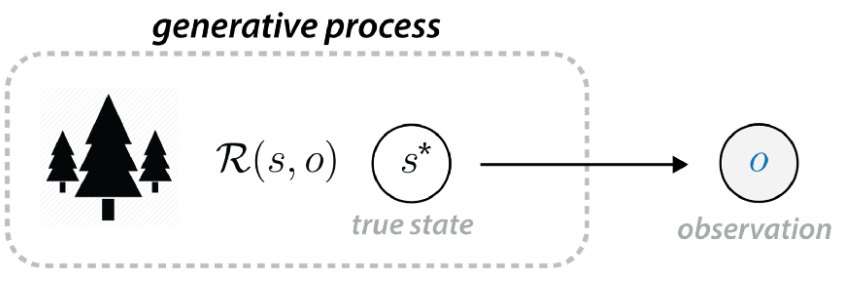
\includegraphics[width=1\linewidth]{one}
		\label{ris:image}
	\end{figure}

	С другой стороны, мозг пытается сделать заключение[infer] о вероятности разных скрытых состояний[states], учитывая наблюдения, $p(s|o)$. И делает он это через приорные знания[prior belief] $p(s)$ и правдободобие[likelihood] $p(o|s)$. Таким образом, мозг строит генерируемый процесс[generative process] определяемую as a joint $p(s,o)$.

	\begin{figure}[h]
		\center{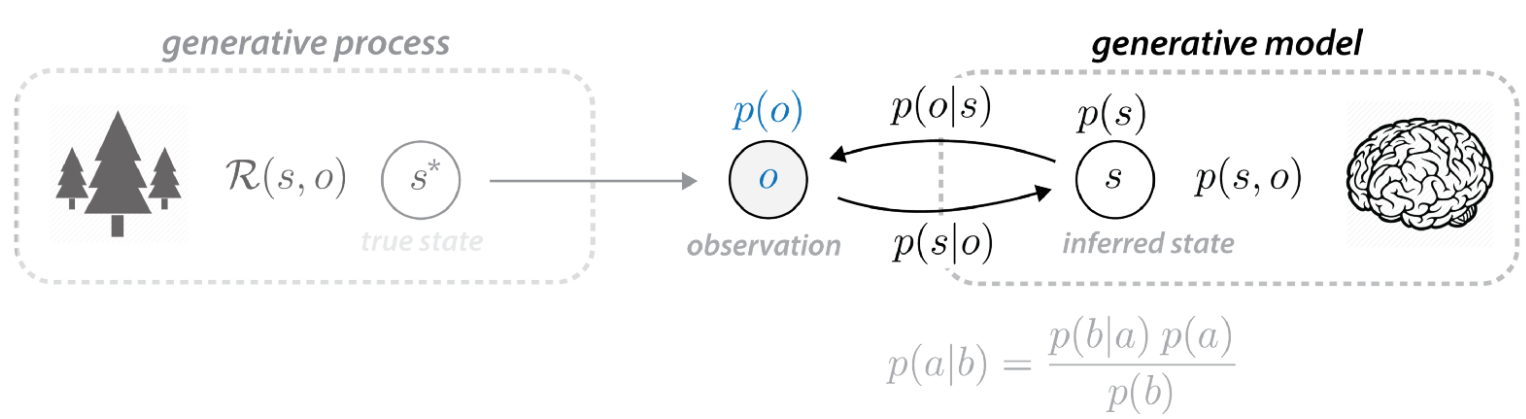
\includegraphics[width=1\linewidth]{two}}
		\label{ris:image}
	\end{figure}

	Давайте рассмотрим пример. Представим следующий генерируемый процесс[generative proces] - в нашем саду яблочное и апельсиновое дерево. Обозначим за скрытую переменную \textbf{s} - является фрукт апельсином или яблоком. Предположим, что яблочное дерево немного левее апельсинового дерева. Итак, когда фрукты падают на землю, мы наблюдаем следующее:

	\begin{figure}[h]
		\center{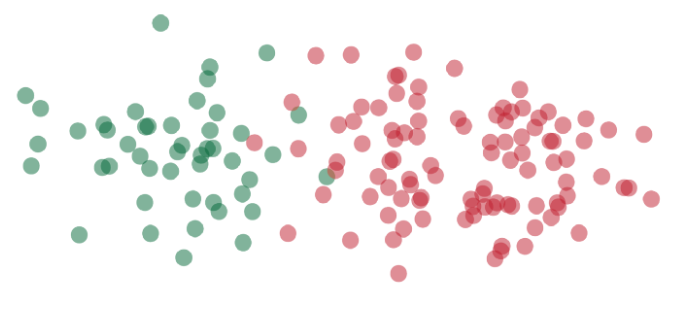
\includegraphics[width=1\linewidth]{three}}
		\label{ris:image}
	\end{figure}

	Кажется, что 70\% лежащих фруктов - апельсины, а остльные 30\% - яблоки. Это истинное[true] распределение скрытого состояния[hidden state] \textbf{s}. Когда фрукты падают, они не попадают в одно и тоже местоположение, они рандомно распространяются вокруг. Это уже вероятность наблюдении при условии \textbf{s}. \textbf{Вывод}[\textbf{Inference}] в генерируемой модели[generative model] заключается в нахождении постериорного[posterior] распределения $p(s|o)$ - вероятность того, что фрукт является яблоком, учитывая его местоположения. \textbf{Обучение}[\textbf{Learning}] генерируемой модели[generative model] состоит из оценивания параметров распределения(таких как, например, математическое ожидание и дисперсия для нормального распределения) скрытого состояния[hidden state] $p(s)$, of the state-observation mapping $p(o|s)$. Вывод $p(s|o)$ через теорему Байеса требует от нас подсчета вероятности $p(o)$, которая интересна собою, учитывая тот факт, что чем лучше наша модель, тем выше будет вероятность наблдаемой информации[observed data] $p(o)$. Это также называется 1) 'model evidence', так как это учитывает как хорошо наша модель предсказывает настоящие данные[real data], 2) 'marginal likelihood',  because we marginalize, or sum out, the hidden state s.
	Сравним 2 модели внизу, которые оценивают $p(o,s)$: модель слева, очевидно, лучше - $p(s)$ корректно показывает, что апельсинов больше, чем яблок, и $p(o|s)$ хорошо центрирован по всем кластерам. Мы можем количественно оценить качество каждой модели с помощью свидетельства модели $p(o)$, изолируя скрытую переменную s.
	
	%\begin{figure}[h]
	%	\center{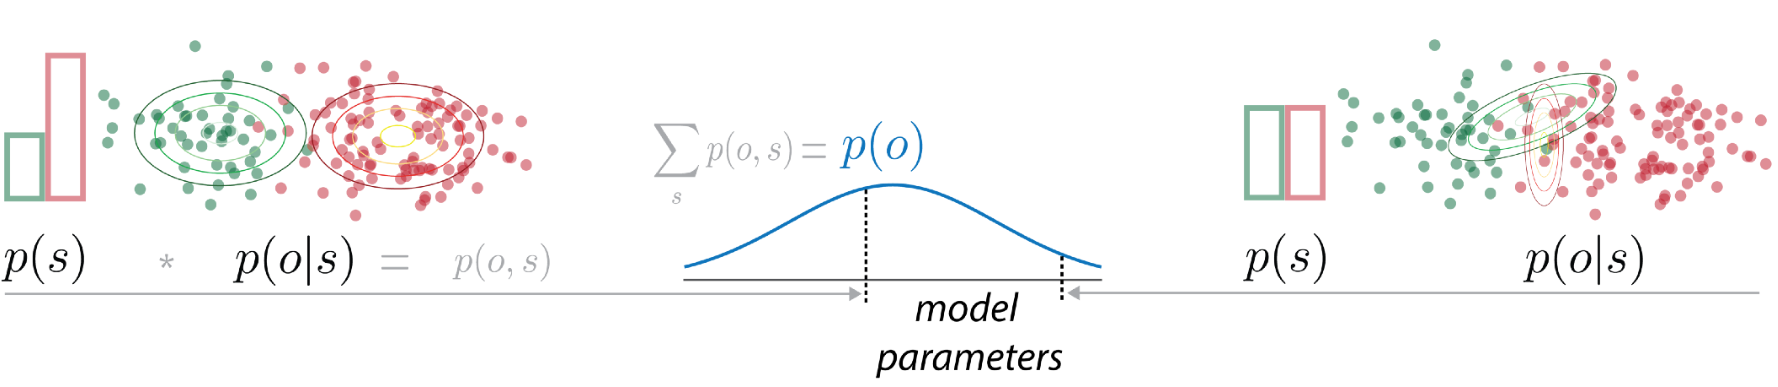
\includegraphics[width=1\linewidth]{four}}
	%	\label{ris:image}
	%\end{figure}

	В идеале, мы хотим выбрать такие параметры модели, которые будут вести к насколько возможно лучшему model evidence $p(o)$. Как это связано с активным выводом[active inference] и с агентом, который избегает неожиданных наблюдений? По факту, задача \textbf{максимизации model evidence эквивалентна минимизации неожиданности}, которая всего лишь отрицательный логарифм $p(o)$. Если вероятность равна 1 - неожиданность[surprise] равна 0, вероятность равна 0 - неожиданность[surprise] стремится к бесконечности. Здесь неожиданность[surprise] представлена, как функция от вероятности:
	
	%\begin{figure}[h]
	%	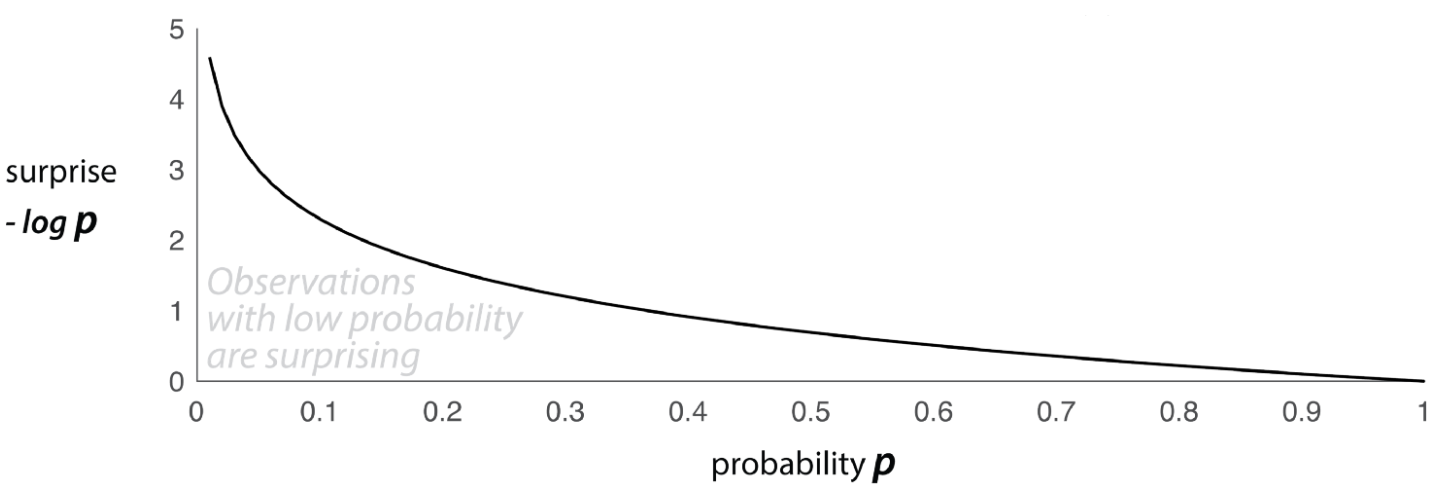
\includegraphics[width=1\linewidth]{five}
	%	\label{ris:image}
	%\end{figure}
	
	Здесь неожиданность[surprise] $-log$ $p(o)$, overlaid с model evidence $p(o)$:
	
	%\begin{figure}[h]
	%	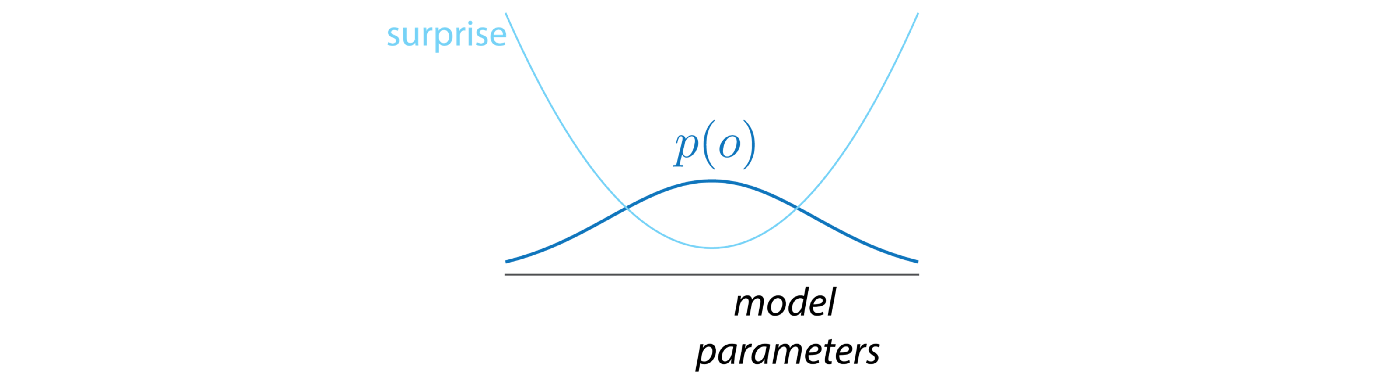
\includegraphics[width=1\linewidth]{six}
	%	\label{ris:image}
	%\end{figure}
	
	Как мы обсуждали выше для model evidence, чтобы оценить неожиданность[surprise] $-log$ $p(o)$, нам  нужно просуммировать по скрытой переменной \textbf{s} совместное распределение $p(o, \textbf{s})$:
	
	%\begin{figure}[h]
	%	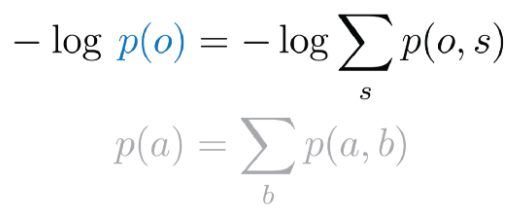
\includegraphics[width=1\linewidth]{seven}
	%	\label{ris:image}
	%\end{figure}
	
	Так как речь идет о суммировании по всем возможным значениям \textbf{s}, суммирование может стать очень тяжелым занятием, если будет очень много различных значений \textbf{s}. Однако есть трюк, который поможет вам избежать невозможного суммирования.
	
	Вместо того, чтобы считать неожиданность[surprise] прямо, мы можем аппроксимировать ее чем-то очень схожим и легко обрабатываемым. Сперва, мы представляем простое распределение[dummy distribution] q с областью значений s (которая окажется безумно полезной позже). Мы можем спокойно внести ее в сумму через деление и умножение одновременно: 
	
	%\begin{figure}[h]
	%	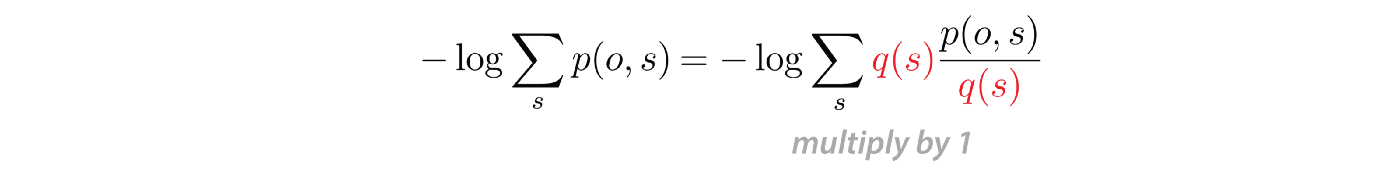
\includegraphics[width=1\linewidth]{eight}
	%	\label{ris:image}
	%\end{figure}
	
	Это дает нам взвешенную сумму, в которой для каждой s, отношение $p(o, s)/q(s)$ суммируется с весом $q(s)$. Это все еще та же неожиданность[surprise] $-log$ $p(o)$, но теперь нам очень удобно ее изменить аппроксимированием.
	
	Теперь же, давайте отвлечемся от неожиданности[surprise] на секунду и сфокусируемся на аппроксимировании. Мы знаем, что функция неожиданности[surprise] $-log$ выглядит как впадина или чаша(иными словами выпуклая). Определение гласит: функция выпуклая в том случае, если когда вы уроните на нее палку, палочка окажется в функции, как в миске. Формально мы объясняем это следующим образом. Давайте возьмем 2 точки на оси абсцисс (\textbf{x} и \textbf{y}), и выберем число между 0 и 1 (\textbf{w}). Как показано ниже, мы можем двигаться между \textbf{x} и \textbf{y} с помощью их взвешенной суммы через изменение \textbf{w} от 0 до 1. То есть мы могли бы рассматривать \textbf{w} и (1 - \textbf{w}) как параметры обычного распределения[simple distribution]. На самом деле, есть краткое название для «взвешенных сумм, в которых веса определяются распределением» - \href{https://en.wikipedia.org/wiki/Expected_value}{математическое ожидание}. Теперь вернемся к тетиве в луке: если вы оцениваете функцию этого ожидания, она всегда будет ниже или равна ожиданию функции, оцененной в \textbf{x} и \textbf{y}.
	
	%\begin{figure}[h]
	%	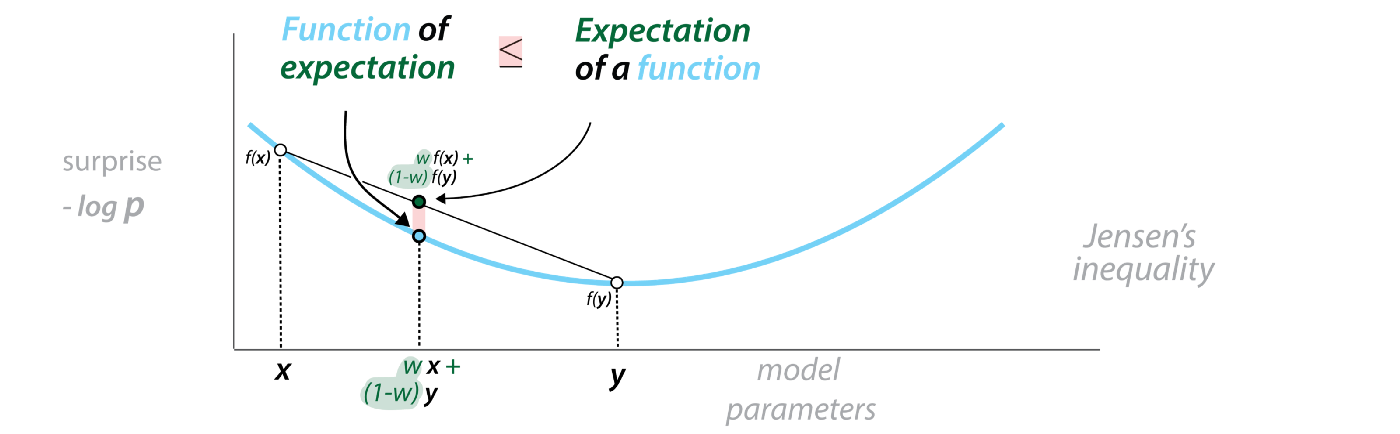
\includegraphics[width=1\linewidth]{nine}
	%	\label{ris:image}
	%\end{figure}
	
	Поскольку ранее мы обозначили неожиданность[surprise], как функцию (-log) от математического ожидания (взвешенной суммы отношения $p(o, s) / q(s)$), то неравенство выпуклости[inequality of convexity] выглядит подходящей для нашего приближения! Формально, это называется «верхняя граница». И вот, эта верхняя граница... Свободная энергия.
	
	%\begin{figure}[h]
	%	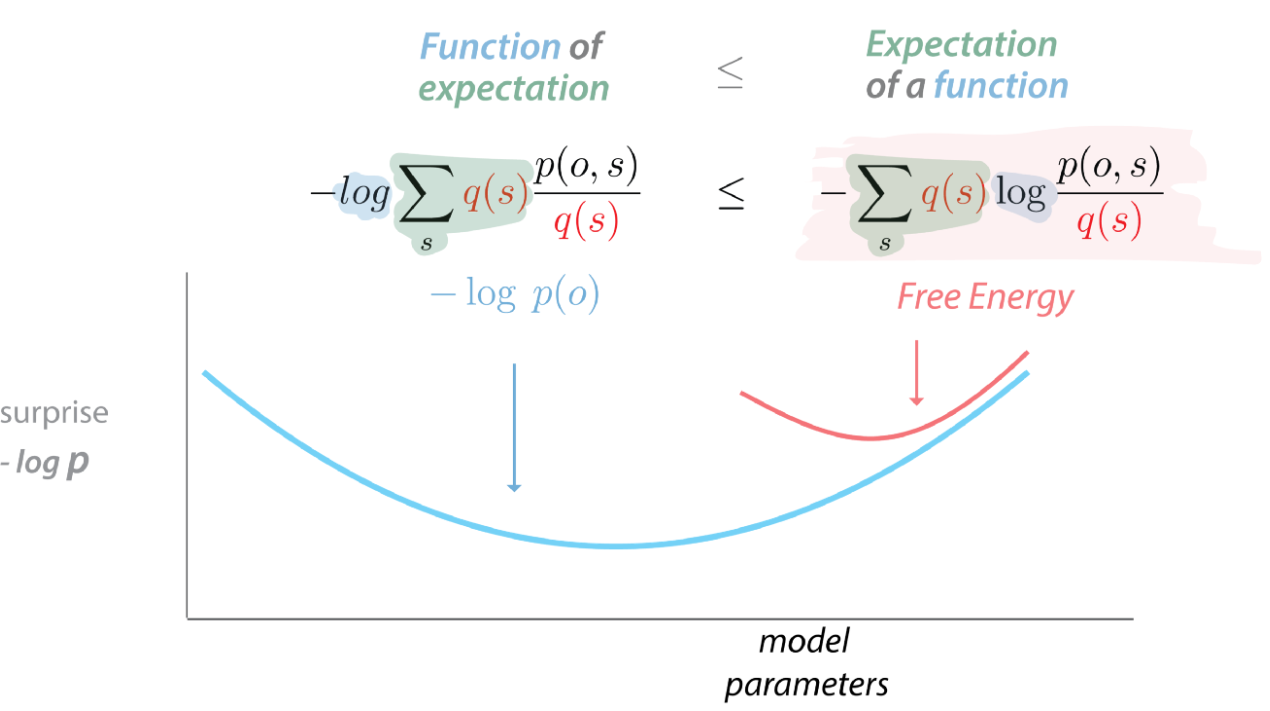
\includegraphics[width=1\linewidth]{ten}
	%	\label{ris:image}
	%\end{figure}
	 
	Мы можем пойти на шаг дальше и убрать минус перед логарифмом. Это приведет нас к определению, которое используют в статьях про Актинвный Вывод[Active Inference]:
	
	%\begin{figure}[h]
	%	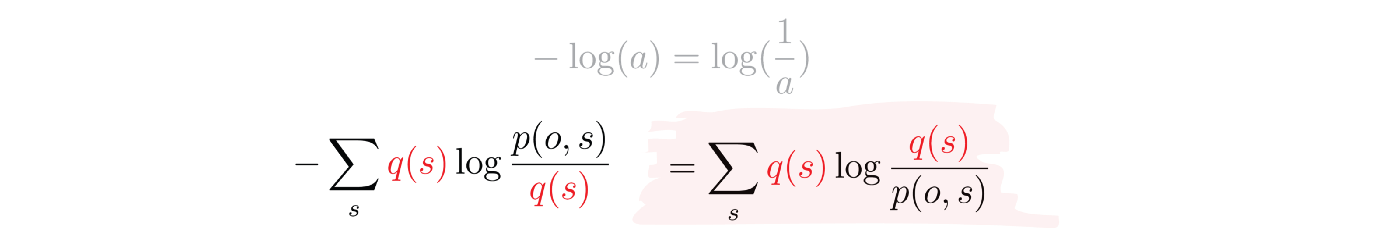
\includegraphics[width=1\linewidth]{eleven}
	%	\label{ris:image}
	%\end{figure}

	Крутая вещь в Свободной Энергии заключается в том, что веса в суммировании определяются \textbf{q(s)}, и мы имеем полный контроль над $q(s)$. Получается, что мы можем покачивать $q(s)$ таким образом, чтобы минимизировать свободную энергию.
	
	Используя пару стандартных идентификаторов, Свободная Энергия[Free Energy] (обычно добавляемая в литературе как «Variational») может быть разложена двумя эквивалентными способами.
	
	%\begin{figure}[h]
	%	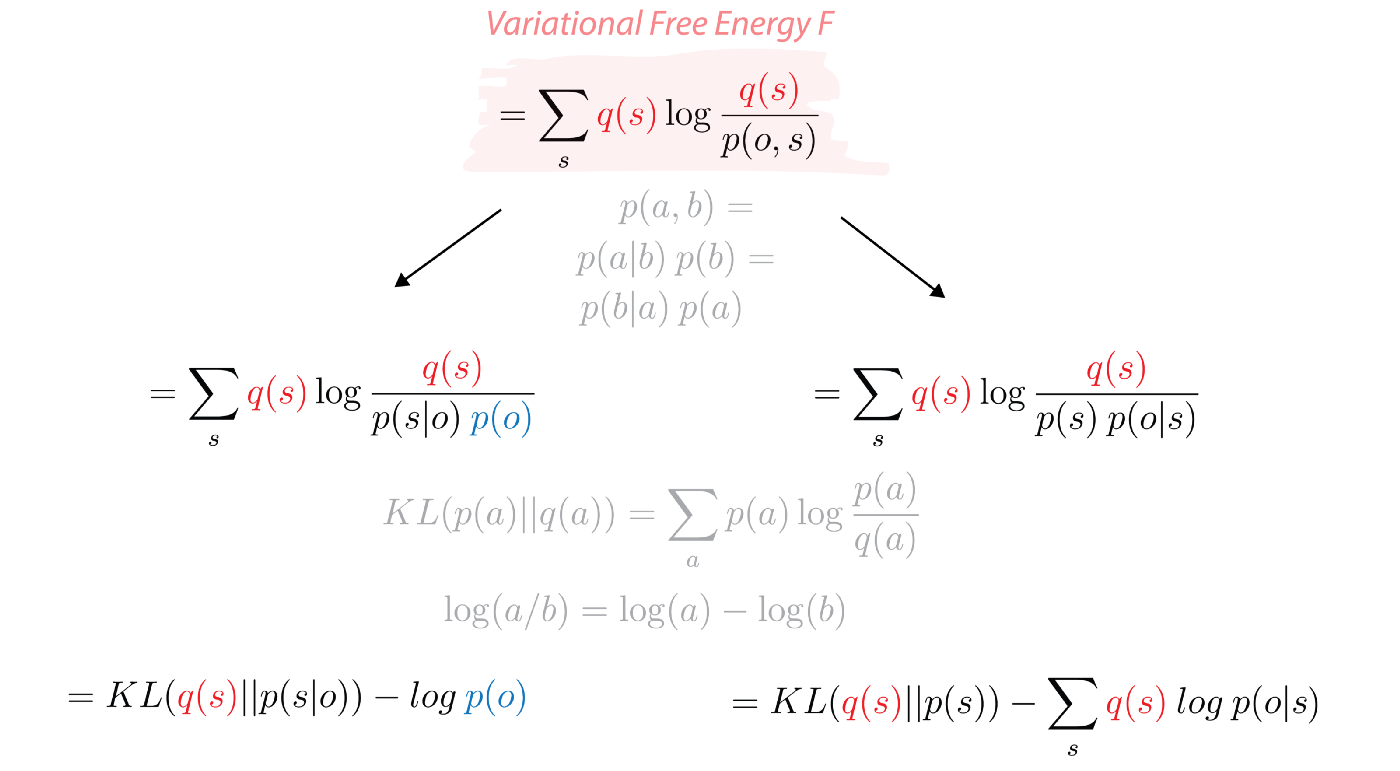
\includegraphics[width=1\linewidth]{twelve}
	%~	\label{ris:image}
	%\end{figure}
	
	Хотя правая ветвь обычно используется на практике, давайте сосредоточимся на левой, так как она дает нам хорошее теоретическое понимание [примечание: мы можем убрать ожидание (сумму по s из $q(s)$) перед $-log$ $p(o)$, поскольку $p(o)$ не зависит от s, а $q(s)$ как распределение вероятностей суммируется до 1]. Это говорит о том, что свободная энергия равна дивергенции KL (Кульбака - Лейблера) между $q(s)$ и $p(s|o)$, и сюрпризу $-log$ $p(o)$.
	
	%\begin{figure}[h]	
	%	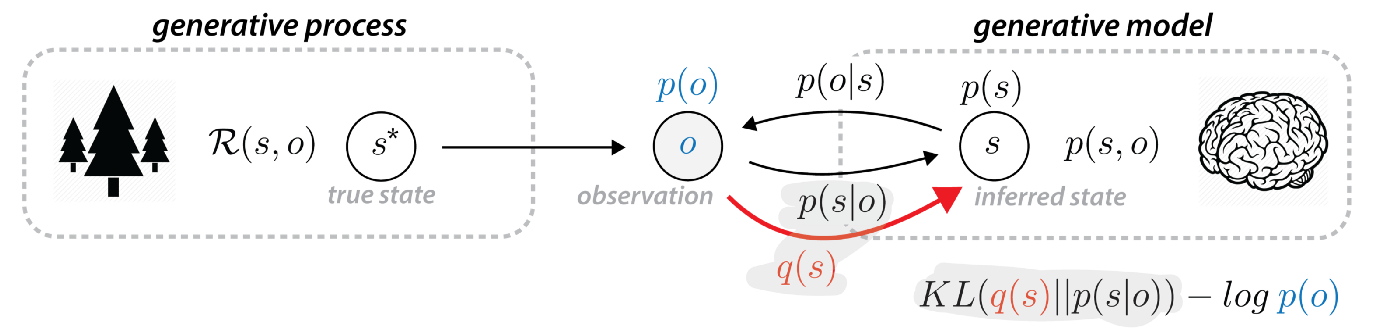
\includegraphics[width=1\linewidth]{thirteen}
	%	\label{ris:image}
	%\end{figure}
	
	Таким образом, минимизируя свободную энергию, произвольное распределение $q(s)$ становится ближе к постериорному $p(s|o)$, и если они совпадают, дивергенция KL становится равной 0, а свободная энергия точно равна неожиданности[surprise]. Таким образом, чем больше мы минимизируем свободную энергию путем покачивания $q(s)$, тем ближе она становится к неожиданности[surprise] (поскольку это верхняя граница), а путем минимизации свободной энергии путем, покачивания параметров $p(o,s)$ мы можем минимизировать неожиданность[surprise] еще больше. Это подробно показано в  \href{https://medium.com/@solopchuk/intuitions-on-predictive-coding-and-the-free-energy-principle-3fc5bcedc754}{посте о прогнозирующем кодировании[pedictive coding]}, которое является следствием принципа свободной энергии, применяемого к восприятию. Вот краткое изложение на данный момент: минимизируем приближение к неожиданности (свободную энергию) $\Rightarrow$ избегаем неожиданных наблюдений $\Rightarrow$ избегаем неожиданных состояний[states] $\Rightarrow$ поддерживаем гомеостазис $\Rightarrow$ остаемся живыми.
	
	До сих пор мы имели дело со статической ситуацией, с одним скрытым состоянием и одним набором наблюдений, но реальный мир динамичен. Таким образом, у нас будет скрытое состояние в каждый момент времени, и, поскольку все имеет тенденцию зависеть от того, \textbf{что произошло раньше}, мы будем предполагать, что s в определенный момент времени t зависит от s в предыдущий момент времени. Например, вероятность увидеть радугу напрямую зависит от того, шел ли дождь раньше.
	
	%\begin{figure}[h]	
	%	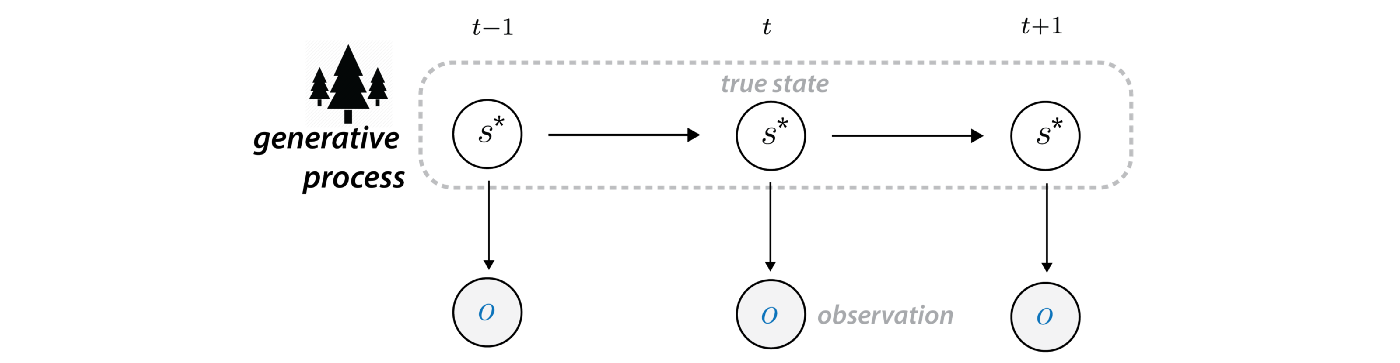
\includegraphics[width=1\linewidth]{fourteen}
	%	\label{ris:image}
	%\end{figure}
	
	Как и прежде, мы пытаемся смоделировать истинный генерируемый процесс[true generative process], изучая генерируемую модель[generative process] $p(o,s)$ и получая приближение к постериорным $q(s)$ на каждом временном шаге. Как и в простой статической ситуации, мы можем найти, каким образом нужно изменить параметры $p(o,s)$ и $q(s)$, чтобы уменьшить свободную энергию, а затем сделать много маленьких шагов в этом направлении.

	%\begin{figure}[h]	
	%	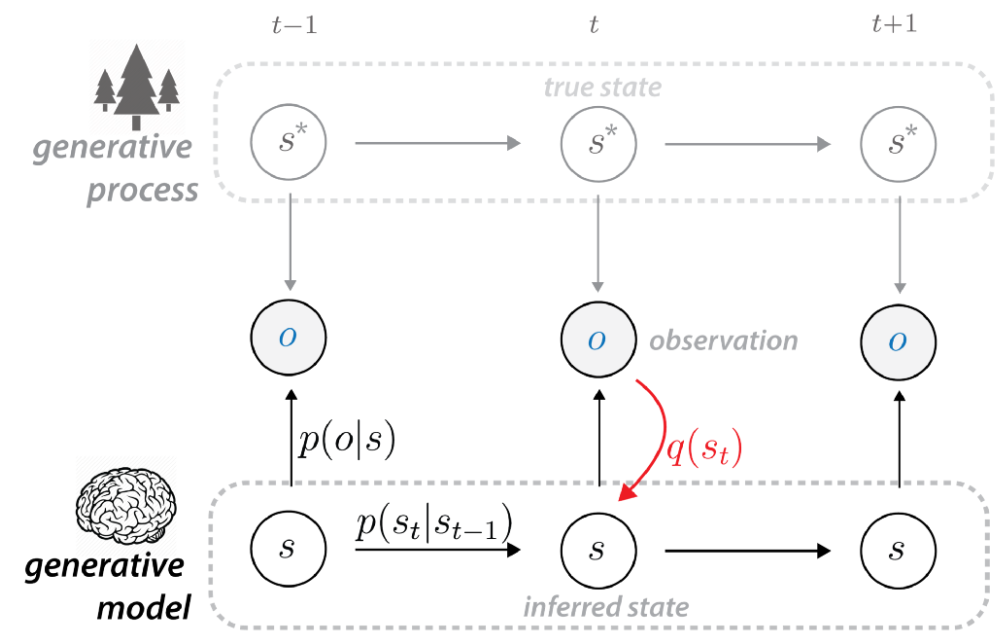
\includegraphics[width=1\linewidth]{fifteen}
	%	\label{ris:image}
	%\end{figure}

	Это будет работать, но мы просто будем пассивно наблюдать за окружающей средой. Что если мы тоже будем воздействовать на нее? В этом случае s в определенный момент времени t будет зависеть от s в предыдущий момент времени и нашего действия u. Другими словами, действие может напрямую влиять на состояние мира, поэтому другое действие может привести к иному будущему (например, мы можем физически двигать вещи своими действиями).

	%\begin{figure}[h]	
	%	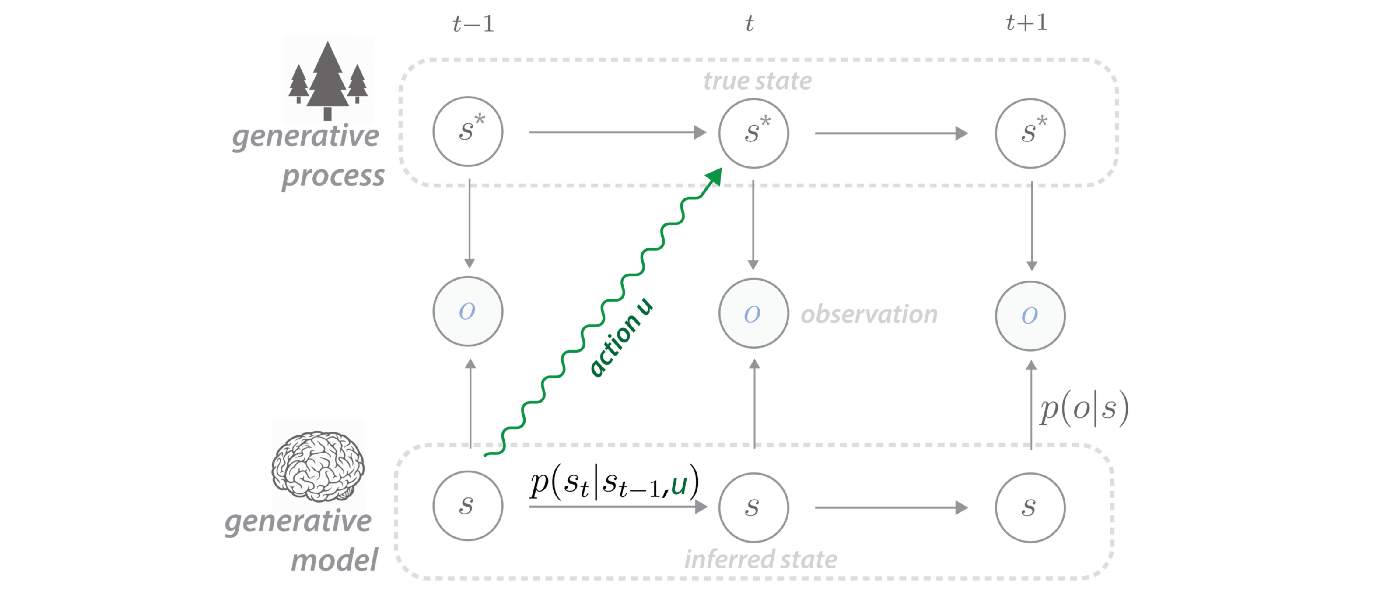
\includegraphics[width=1\linewidth]{sixteen}
	%	\label{ris:image}
	%\end{figure}

	Теперь вывод становится активным[inference becomes active]! Нам просто нужно найти способ выбрать хорошее действие на каждом временном шаге. В действительности кажется, что мы не рассматриваем последствия действий только на следующем временном шаге․ Мы планируем всю политику, серию действий, ориентированных на отдаленные во времени цели. Поэтому, если есть много возможных действий и много будущих моментов времени $\Rightarrow$ есть много потенциальных политик, которые мы можем предпринять. Активный вывод говорит: просто рассмотрите все варианты. Таким образом, мы делаем вывод, аппроксимируя $p(s|o)$ с $q(s)$ одновременно (параллельно) для каждой возможной политики \pi.

	%\begin{figure}[h]	
	%	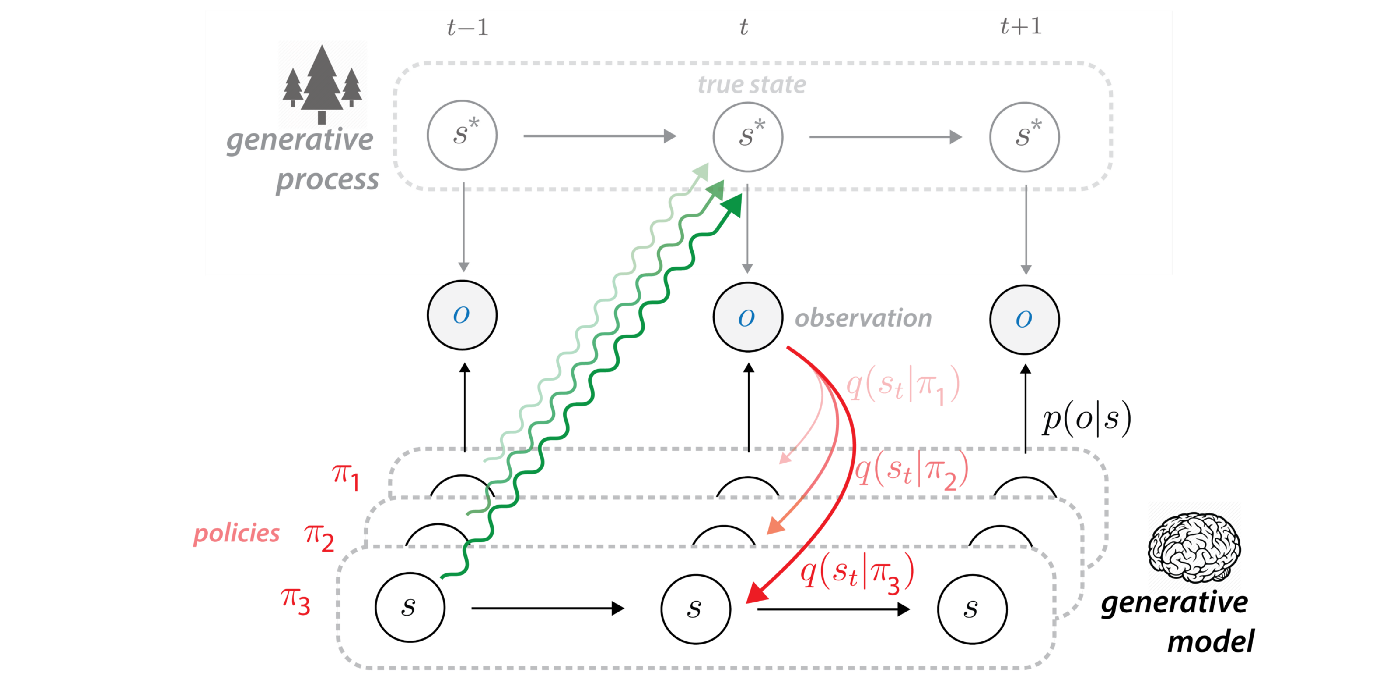
\includegraphics[width=1\linewidth]{seventeen}
	%	\label{ris:image}
	%\end{figure}

	И поскольку наша цель остается прежней - минимизировать неожиданность[surprise] путем минимизации свободной энергии[free energy] - мы можем вычислить свободную энергию[free energy] (и направление изменения $q(s)$, которое минимизирует FE) при каждом возможном шаге политики и времени.
	
	\textbf{Политики(имеется в виду планы)[Policies], которые минимизируют Свободную Энергию[Free Energy] в будущем, являются предпочтительными}. Допустим, мы планируем на 10 временных шагов вперед. Если мы находимся в момент времени t = 1, для каждой политики мы суммируем Свободные энергии для шагов с 1 по 10 времени и выбираем политику, которая имеет минимальную кумулятивную Свободную энергию в будущем. Давайте еще раз посмотрим на общую картину того, как можно рассчитать свободную энергию:
	
	%\begin{figure}[h]	
	%	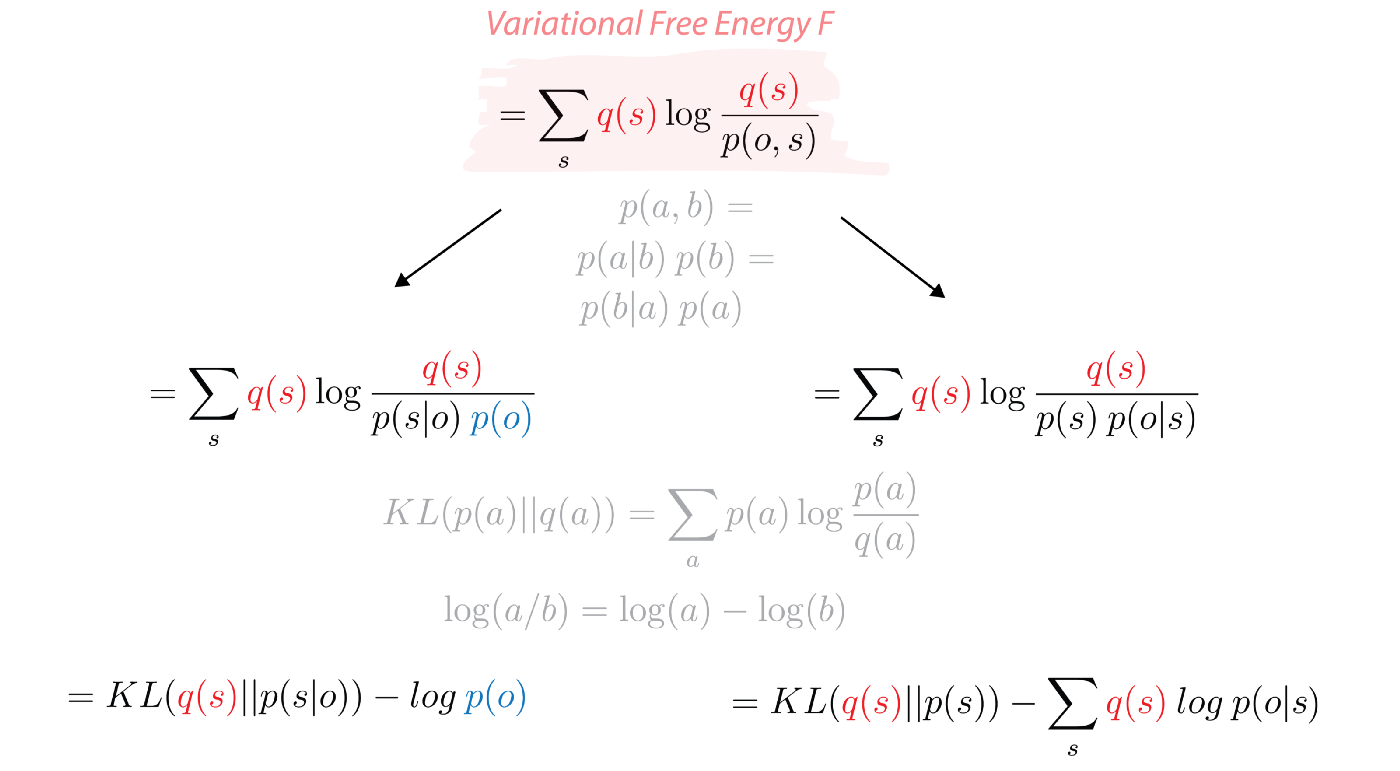
\includegraphics[width=1\linewidth]{eightteen}
	%	\label{ris:image}
	%\end{figure}

	Левая ветвь показывает нам важные теоретические свойства минимизации свободной энергии (например, что $q(s)$ приближается к $p(s|o)$), но это нецелесообразно, поскольку мы используем свободную энергию для аппроксимации $-log$ $p(o)$ в первую очередь. Итак, давайте посмотрим на правую ветвь, которая является стандартным способом вычисления свободной энергии:
	
	%\begin{figure}[h]	
	%	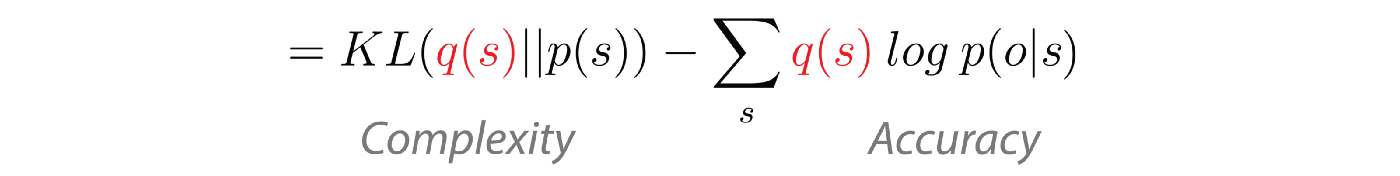
\includegraphics[width=1\linewidth]{nineteen}
	%	\label{ris:image}
	%\end{figure}

	Эти два термина обычно называют сложностью[complexity] и точностью[accuracy]. Сложность[Complexity] показывает, насколько аппроксимация апостериорного $q(s)$ отклоняется от приорного $p(s)$, и количественно определяет, сколько дополнительных битов информации, которых нет в приорном распределении, мы хотим закодировать в приблизительном апостериорном $q(s)$. Точность[Accuracy] (ожидаемое значение $p(o|s)$) оценивает вероятность того, что состояниям дан конкретный результат o. Хотя мы можем легко вычислить Сложность[Complexity], существует проблема в оценке Точности[Accuracy] для будущих временных шагов - просто потому, что мы еще не наблюдали результаты. Таким образом, нам нужен другой способ вычисления свободной энергии[free energy], поэтому мы пойдем по левой ветви разложения FE. Но здесь есть одна загвоздка: поскольку у нас нет доступа к будущим наблюдениям - нам нужно угадать, как они могли бы выглядеть, и взять взвешенную сумму свободной энергии по догадкам $p(o|s)$. Обратите внимание, что мы будем ставить вероятности на \pi, так как свободная энергия оценивается отдельно для каждой политики. Предполагается, что только отображение наблюдения состояния $p(o|s)$ одинаково для всех политик.
	
	%\begin{figure}[h]	
	%	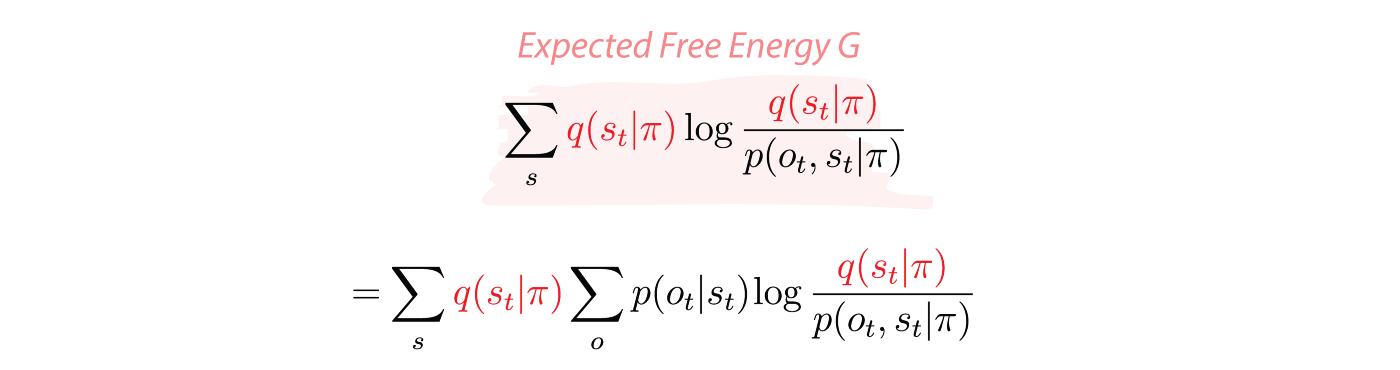
\includegraphics[width=1\linewidth]{twenty}
	%	\label{ris:image}
	%\end{figure}

	

\end{document}]